\documentclass[tikz,border=3pt]{standalone}
% Shared style for every figure: one font (Latin Modern), one block vocabulary, token colours.
\usepackage{fontspec}
\usepackage{unicode-math}
\setmathfont{latinmodern-math.otf}
\usetikzlibrary{arrows.meta,positioning,fit,calc,backgrounds,shapes.misc,decorations.pathreplacing}
% Token colours: exact RGB codes, remapped to CSS variables after conversion (see tokens in svgfix.py)
\definecolor{ink}{RGB}{0,0,0}
\definecolor{inkb}{RGB}{90,90,90}
\definecolor{grid}{RGB}{200,200,200}
\definecolor{paper}{RGB}{255,255,255}
\definecolor{fdata}{RGB}{231,238,246}
\definecolor{fmodel}{RGB}{246,238,224}
\definecolor{ftarget}{RGB}{232,243,234}
\definecolor{fpub}{RGB}{248,233,226}
\definecolor{own}{RGB}{42,120,214}
\definecolor{pub}{RGB}{235,104,52}
\tikzset{
  >={Latex[length=1.9mm,width=1.5mm]},
  every picture/.style={line width=0.5pt, ink, font=\normalsize},
  blk/.style={draw=ink, rounded corners=1.2pt, align=center, inner xsep=5pt, inner ysep=4pt, minimum height=9mm, fill=paper},
  data/.style={blk, fill=fdata},
  model/.style={blk, fill=fmodel},
  target/.style={blk, fill=ftarget},
  pubm/.style={blk, fill=fpub},
  op/.style={draw=ink, circle, inner sep=1.2pt, fill=paper, font=\small},
  group/.style={draw=inkb, dashed, rounded corners=2pt, inner sep=6pt},
  glabel/.style={font=\small\scshape, text=inkb, inner sep=1pt},
  note/.style={font=\footnotesize, text=inkb, align=center, inner sep=1pt},
  wt/.style={font=\footnotesize, fill=paper, inner sep=1pt},
  flow/.style={->, draw=ink},
  dflow/.style={->, draw=inkb, dashed},
}

\begin{document}
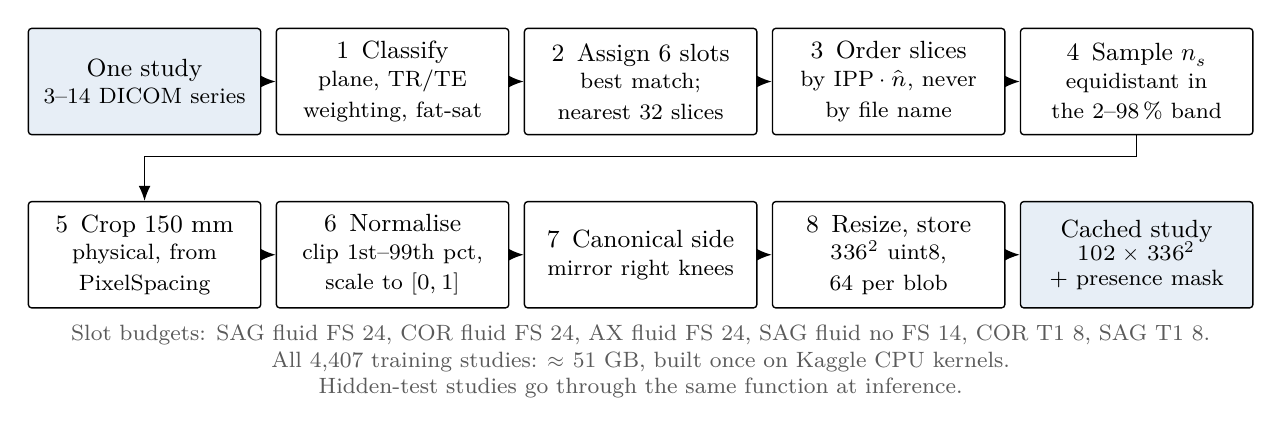
\begin{tikzpicture}[font=\small]
\tikzset{blk/.append style={text width=2.6cm, minimum height=1.35cm}}
\def\dx{3.15}
\node[data] (in) at (0,0) {One study\\[-1pt]{\footnotesize 3--14 DICOM series}};
\node[blk] (s1) at (\dx,0)  {1\enspace Classify\\[-1pt]{\footnotesize plane, TR/TE weighting, fat-sat}};
\node[blk] (s2) at (2*\dx,0)  {2\enspace Assign 6 slots\\[-1pt]{\footnotesize best match; nearest 32 slices}};
\node[blk] (s3) at (3*\dx,0)  {3\enspace Order slices\\[-1pt]{\footnotesize by $\mathrm{IPP}\cdot\hat n$, never by file name}};
\node[blk] (s4) at (4*\dx,0) {4\enspace Sample $n_s$\\[-1pt]{\footnotesize equidistant in the 2--98\,\% band}};
\node[blk] (s5) at (0,-2.2)  {5\enspace Crop 150 mm\\[-1pt]{\footnotesize physical, from PixelSpacing}};
\node[blk] (s6) at (\dx,-2.2)  {6\enspace Normalise\\[-1pt]{\footnotesize clip 1st--99th pct, scale to $[0,1]$}};
\node[blk] (s7) at (2*\dx,-2.2)  {7\enspace Canonical side\\[-1pt]{\footnotesize mirror right knees}};
\node[blk] (s8) at (3*\dx,-2.2)  {8\enspace Resize, store\\[-1pt]{\footnotesize $336^2$ uint8, 64 per blob}};
\node[data] (out) at (4*\dx,-2.2) {Cached study\\[-1pt]{\footnotesize $102\times336^2$\\[-2pt]+ presence mask}};
\draw[flow] (in) -- (s1);
\draw[flow] (s1) -- (s2); \draw[flow] (s2) -- (s3); \draw[flow] (s3) -- (s4);
\draw[flow] (s4.south) -- ++(0,-0.27) -| (s5.north);
\draw[flow] (s5) -- (s6); \draw[flow] (s6) -- (s7); \draw[flow] (s7) -- (s8);
\draw[flow] (s8) -- (out);
\node[note, anchor=north] at (2*\dx,-3.05) {Slot budgets: SAG fluid FS 24, COR fluid FS 24, AX fluid FS 24, SAG fluid no FS 14, COR T1 8, SAG T1 8.\\All 4,407 training studies: $\approx$ 51 GB, built once on Kaggle CPU kernels.\\Hidden-test studies go through the same function at inference.};
\end{tikzpicture}
\end{document}
